\documentclass[10pt, twocolumn]{article}

\usepackage{times,url}
\usepackage{multirow}
\usepackage{tabularx}
\usepackage{amsmath}
\usepackage{rotating}
\usepackage{xcolor}
\usepackage{array}

\usepackage[sort]{cite}

\makeatletter
\newcommand*{\rom}[1]{\expandafter\@slowromancap\romannumeral #1@}
\makeatother

\def\Section {\S}

\newtheorem{theorem}{Theorem}[section]
\newtheorem{observation}[theorem]{Observation}
\newtheorem{lemma}[theorem]{Lemma}
\newtheorem{proposition}[theorem]{Proposition}
\newtheorem{corollary}[theorem]{Corollary}

\newenvironment{definition}[1][Definition]{\begin{trivlist}
\item[\hskip \labelsep {\bfseries #1}]}{\end{trivlist}}
\newenvironment{example}[1][Example]{\begin{trivlist}
\item[\hskip \labelsep {\bfseries #1}]}{\end{trivlist}}
\newenvironment{remark}[1][Remark]{\begin{trivlist}
\item[\hskip \labelsep {\bfseries #1}]}{\end{trivlist}}

% Macros:
\newcommand{\ie}{{\it i.e.}}
\newcommand{\eg}{{\it e.g.}}
\newcommand{\cf}{{\it cf.}}
\newcommand{\etc}{{\it etc.}}
\newcommand{\viz}{{\it viz.}}
\newcommand{\apriori}{{\it a priori}}
\newcommand{\eat}[1]{}

% Notes:
\newcommand{\num}[1]{{\color{red}\bf {#1}}}

\newcommand{\giulia}[1]{{\color{red} {#1}~(Giulia)}}
\newcommand{\wenting}[1]{{\color{blue}{#1}~(Wenting)}}


% Signed quotes:
\def\signed #1{{\leavevmode\unskip\nobreak\hfil\penalty50\hskip2em
  \hbox{}\nobreak\hfil(#1)%
    \parfillskip=0pt \finalhyphendemerits=0 \endgraf}}

\newsavebox\mybox
\newenvironment{aquote}[1]
  {\savebox\mybox{#1}\begin{quote}}
    {\signed{\usebox\mybox}\end{quote}}

\sloppy
\begin{document}

\title{Deanonymizing Anonymous Messaging Social Networks}

\author{Giulia Fanti and Wenting Zheng}

   \date{}
   \maketitle
   \thispagestyle{empty}
\section{Introduction}
In recent years, anonymous messaging applications like Whisper and Secret have gained popularity. These services spread messages to users’ friends without including any authorship information. In this project, we wish to explore whether a third-party adversary, e.g., local law enforcement, can deanonymize messages by simply participating in the network and knowing the underlying social graph. 

We believe this may be possible due to a recent body of work on locating the patient-zero for a disease spreading over a graph \cite{shah2011rumors}. In our case, the “disease” corresponds to a message, and nodes are ``infected” once they observe the message. Existing work assumes that the estimator can uniformly sample the graph to learn a subset of the infected nodes; given this, there exist strong guarantees and tractable methods for inferring an infection source.

In our case, ``sampled nodes” are nodes corrupted by the adversary, such that they can see the time and content of all messages reaching that node, but do not actively alter the protocol. Corrupted nodes could be either directly colluding with the adversary, or they might be spambots that create artificial friendship links with the sole purpose of monitoring network activity. Due to the patterns of false-friend creation, we believe that such corrupted nodes are unlikely to be uniformly dispersed across the graph. 

In this work, we wish to study two questions: 1) How many legitimate nodes (i.e., corresponding to real people) must an adversary corrupt in order to reliably deanonymize users? 2) How should an adversary select spies in order to maximize the probability of finding the sources of messages? We believe we can show through simulation that networks are susceptible to deanonymization by adversaries with limited power to create friendships and/or corrupt nodes.



\section{Related Work}

\subsection{Anonymous Social Networks} 
Recent years have seen the rise of a new class of social network built upon anonymous microblogging.
Such networks, including Secret \cite{secret}, Whisper \cite{whisper}, and Yik Yak \cite{yikyak}, enable users to share short messages with their friends without including any authorship information in the metadata. 
Whenever a user `likes' an incoming message, that message passes to the user's friends.
Under this spreading pattern, messages propagate across the network like an epidemic.
While content on these social networks is anonymous to individual network users, service providers store all communications (and authorship information) on centralized servers.
The networks are therefore not anonymous to service providers themselves, as well as government agencies or hackers who obtain access to these centralized servers.
Our work considers a different adversary that is more powerful than a single user, but less powerful than a government agency or service provider.
%Because this class of social networks is relatively new, to the best of our knowledge, no existing research exists on deanonymizing them.

These social networks are not the gold standard for anonymous communication. In the rest of this section, we will discuss the state-of-the-art in anonymous broadcast communication, and explain why those methods have not gained traction outside the research community.
A wide swath of literature---spanning a few decades---considers the problem of communicating anonymously.
Much of this work focuses on \emph{point-to-point} communication, offering properties like sender anonymity, receiver anonymity, and/or sender-receiver unlinkability. 
Work in this area includes Chaum's mix-nets \cite{chaum1981untraceable}, Tor \cite{tor}, Tarzan \cite{tarzan}, Crowds \cite{reiter1998crowds}, and Herbivore \cite{goel2003herbivore}, just to name a few.
While this body of literature has been very impactful, it is different from our problem of interest.

We instead focus on approaches that enable anonymous \emph{broadcast} communication.
Chaum's seminal work on the dining cryptographers problem launched this area of study \cite{chaum88}.
The problem is as follows: a group of cryptographers goes out to dinner. After the meal, they want to learn if one of them has paid the check, without revealing who paid.
Chaum's solution, known colloquially as a DC-net, requires parties to share secrets with their neighbors and publish a function of those secrets. %requires each cryptographer to flip a coin (in private) with the individuals on his left and right. Each coin flip is hence observed by exactly two people.
%Then, each cryptographer publishes the XOR of the two observed coin flips; if cryptographer Alice paid the check, then instead of publishing the true XOR of her coin flips, she publishes the opposite (e.g., a 0 instead of a 1).
To learn the desired information, each cryptographer computes a function of all the published information. %If nobody paid the check, this bitwise sum will evaluate to 0; otherwise it will evaluate to 1.
DC-nets offer perfect anonymity, but they rely on some assumptions that may not realize in practice, such as the participants being honest, or only one individual communicating at once.

Chaum's work on DC-nets launched a great deal of study on robust, scalable, and anonymous broadcast communication. 
Some of this work focuses on developing new anonymity primitives, such as anonymous broadcast encryption \cite{libert2012anonymous, fazio2012outsider}.
Anonymous broadcast encryption aims to send an encrypted message such that only a subset of recipients can decrypt the message, but none of the recipients knows any of the other recipients' identities; in other words, it provides receiver anonymity.
%Classical broadcast encryption schemes require each recipient to know the entire set of intended recipients, which violates recipient anonymity; anonymous broadcast encryption aims to relax this constraint. 
This work is outside our scope, as we are interested in broadcast systems that provide \emph{sender} anonymity.


Another branch of work focuses on refining DC-nets to exhibit better efficiency or robustness properties against threats to protocol security or correctness \cite{waidner1989dining,golle2004dining,corrigan2010dissent}.
For instance, \cite{golle2004dining} proposes non-interactive DC-net constructions that identify misbehaving parties with high probability.
\cite{corrigan2010dissent} extends this work by proposing a DC-net with a \emph{shuffled send} primitive, which helps provide integrity, anonymity, and accountability within the network.
These proposed improvements to DC-nets are fairly efficient, but they are likely to face challenges at an Internet-wide scale.
Advances in the construction of DC-nets have led to various applications, including voting systems \cite{fujioka1993practical,van2010anonymous}, distributed storage \cite{freeHavenProject}, and even point-to-point anonymous messaging \cite{goel2003herbivore}.
The details of these schemes are not important to understanding our current work; the key take-away is that they all use ideas from DC-nets on a relatively small scale.
For instance, Herbivore \cite{goel2003herbivore} is a point-to-point messaging system that uses DC-nets to provide sender anonymity---but only within a small cluster of the network.
Using DC-nets to communicate across an entire network would be massively impractical, due to their vulnerability to Sybils, Byzantines, and denial-of-service attacks.

The body of anonymous broadcast research has not yet found its way into a large-scale, widely-adopted social network. 
Several factors might explain this, including the scalability and security challenges we mentioned, as well as the difficulty of monetizing truly anonymous services.
The end result is that commercial anonymous social networks described earlier, such as Secret and Whisper, have built significant user bases while offering fairly weak anonymity properties.
As such, they present a juicy target for adversaries hoping to learn people's sensitive secrets.
In this work, we study exactly how powerful an adversary must be to deanonymize such a network.

\subsection{Deanonymizing Social Networks}

Researchers have worked on different techniques for deanonymizing social networks. Early approaches on user deanonymization~\cite{novak2004anti,narayanan2006break} come from inferring user identify from public messages sent by these users. For example, an early work~\cite{novak2004anti} analyzed pseudonymous posts on online bulletin boards. The paper uses machine learning techniques and data mining to analyze these posts. These algorithms extract features and detect post similarity, therefore inferring that some aliases are being used by the same user. 

A more sophisticated approach~\cite{backstrom2007wherefore} considers what happens when you have more limited information, such as only information regarding node connections. The paper models the network as a list of nodes and edges. Nodes are anonymized (original IDs replaced with new IDs), while the communication links (graph edges) are preserved. The attackers have a list of target nodes that they wish to compromise.
The attacks presented in this paper assume that the attackers can construct new nodes a network graph $G$ before it is anonymized. These fake nodes attempt to communicate with a list of targeted honest nodes and these communications are recorded as edges. After the graph is anonymized, the attackers will attempt to identify the fake nodes along with the targeted nodes. 
The aim of our project is a little different. We are attempting to deanonymize an online network that is already anonymized to a certain extent when the attack begins. A subset of the nodes in the network are assumed compromised, and the attackers will leverage anonymous messages to reconstruct the social network graph as well as re-identifying nodes. 

One recent~\cite{narayanan2009anonymizing} approach focuses on deanonymizing large scale social networks by developing a very generic re-identification algorithm. Social graph anonymizaion usually consists of releasing some partial information on a \emph{sanitized} version of the graph. 
The attackers are assumed to know some auxiliary information about the original graph $S$. This auxiliary information, designated as $S_{AUX}$, is a different network such that $S_{AUX}$ and $S$ partially overlap. Using the auxiliary information, the attackers can use an algorithm to deanonymize the sanitized version of $S$, $S_{SAN}$.
The algorithm consists of two steps, seed identification and propagation. Seed identification attempt to find a small amount of users that are present both in the anonymized network and the auxiliary graph. The propagation stage is an iterative process that finds new mappings between $S_{SAN}$ and $S_{AUX}$. This paper's analysis is very informative, and the generic algorithm is very applicable. However, it does not attempt to address the issue of tracking specific messages back to their original sources. We attempt to address both the network graph deanonymization (such that it is possible to discover the network connectivity) and the message deanonymization (such that it is possible to find the original source of the message). In addition, we would like to analyze and quantify the extent of the deanonymization spread for different network topology.

\subsection{Identifying a Rumor Source}
Here we discuss work on statistical rumor source inference over graphs; this literature will inform our choice of inference algorithms for identifying the source of a message.
Rumor source inference has been of interest for a long time, but a recent surge of statistical research started with Shah and Zaman \cite{shah2011rumors}. The problem is as follows: An infection is propagating over a graph according to a diffusion random process. 
That is, each infected node infects an uninfected neighbor in an exponentially-distributed amount of time.
Given the underlying graph structure and a single snapshot of the infection pattern at a given time, can the ``patient-zero" be inferred?
The authors propose a metric called \emph{rumor centrality}, which describes the centrality of a node in the infected subgraph.
They present an efficient method for computing rumor centrality and show that when the underlying social network is tree-structured, the node with maximum rumor-centrality is the true patient-zero with high probability. The intuition is that regular, symmetric spreading patterns (like diffusion) tend to place the true source in the center of the infection graph with high probability. 

Subsequent work has examined many variants of this problem. Examples include considering more general graph structures \cite{shah2012rumor} and altering the estimator's data-collection strategy \cite{pinto,karamchandani2013rumor,luo2013identify}.
In these last papers, the estimator samples a subset of infected nodes, and learns the timestamp at which each node first received the infection. 
This is equivalent to our notion of placing ``spies" in the network. 
This follow-up work mainly reinforces the point that under a variety of graph structures and information collection methods, rumor centrality and other heuristic centrality measures can consistently identify the source with high probability. 
These heuristics are therefore good candidates for our own inference problem. 
Another class of research instead develops new estimation techniques based on message-passing \cite{lokhov2014inferring} and spectral methods \cite{fioriti2012predicting}.
Although these methods perform well, their added complexity makes them less well-suited to our purposes.

While this body of work informs our choice of estimators for rumor source identification, it is not guaranteed that these estimators will work well. 
Existing research assumes that samples are taken regularly over the graph. 
In our work, these sampled nodes correspond to spies or Sybil nodes, which exhibit very different topological characteristics than normal social graph nodes \cite{narayanan2009anonymizing}.
The question is whether irregularly-spaced Sybil nodes (which are easy to make) can achieve the same deanonymization accuracy as a uniformly-spaced network of spies (which is difficult to build).

\section{Model}
We model the underlying social network as a graph $\mathcal G(V,E)$, where $V$ denotes the set of vertices, or participants, in the network, and $E$ denotes the set of edges. We assume that some node $v^*$ starts propagating a message at some point in time, and there are $K$ spies, $s_1,\ldots,s_K$. Each spy $s_i$ will collect the timestamp $t_i$ at which it first receives the message.

Each time a node receives the message, it decides whether or not to `like' this message. If a user likes the message, then the message gets spread to that user's friends, whose first impressions will occur with some delay. We model the time delay between a user $i$ liking a message and the user's friend $j$ seeing the message as a random variable $\theta_{ij}$; the $\theta_{ij}$'s, or delays across each edge in the social graph, are assumed to be iid. We do not specify the distribution of $\theta_{ij}$ \emph{a priori}; in principle, this should be informed by measurements of real social network usage.

After a certain point in time, the adversary collects the timing information $t_i$ from all nodes and tries to estimate the true source. Ideally, it would run an optimal estimation algorithm to output the estimated source $\hat v$, but provably optimal estimators are not currently known for general graphs.


\section{Methodology}
A number of factors could impact the efficacy of deanonymization:
\begin{itemize}
\item \textbf{Estimator}: The method of estimation 
\item \textbf{Underlying graph structure}:
\item \textbf{Fraction of spies}: 
\item \textbf{Location of spies}:
\item \textbf{Propagation latency}:
\end{itemize}

\subsection{Estimators}
Since the majority of work in this space is 

\section{Results}
\subsection{Estimator validation}
We started by attempting to replicate the estimator results in \cite{pinto}. 
In this replication process, we ran into a number of challenges. We encountered four primary mistakes or omissions in \cite{pinto} that affected our estimation accuracy; some of these were easy to correct once we identified them, others were not:
\begin{itemize}
\item There is a typo in equation (2), which describes how to compute the observed delay vector. It should say $[\boldsymbol d]_k=t_{k+1}-t_1$ instead of $[\boldsymbol d]_k=t_{k+1}-t_k$. This is a critical mistake in the description of the estimator that leads to incorrect likelihoods. 
\item Algorithm 2 of the supplemental materials describes how to compute likelihoods for general graphs. In step 6, it should say ``compute the source likelihood using equation (4) for node $s$.", rather than ``using equation (7)." This is because over general graphs, the covariance matrix $\Lambda_s$ is not identical for all nodes, which causes the simplifications in equation (7) to be invalid. As such, the likelihoods should be computed using the more general equation (4). This error initially led to incorrect likelihood computations in our code.
\item Algorithm 2 of the supplemental materials does not explain how to prune graphs that are not tree-structured. Additionally, it does not describe how to incorporate the direction of infection into estimation. These omissions collectively have a significant impact the likelihoods obtained by the algorithm, and we suspect this is partially responsible for our inability to exactly reproduce their results.
\item The parameter specifications of the random graphs in Table 1 are not given. Specifically, the Barabasi-Albert parameter is not given. We therefore tried a range of different parameters.
\end{itemize}

\begin{figure}
\centering
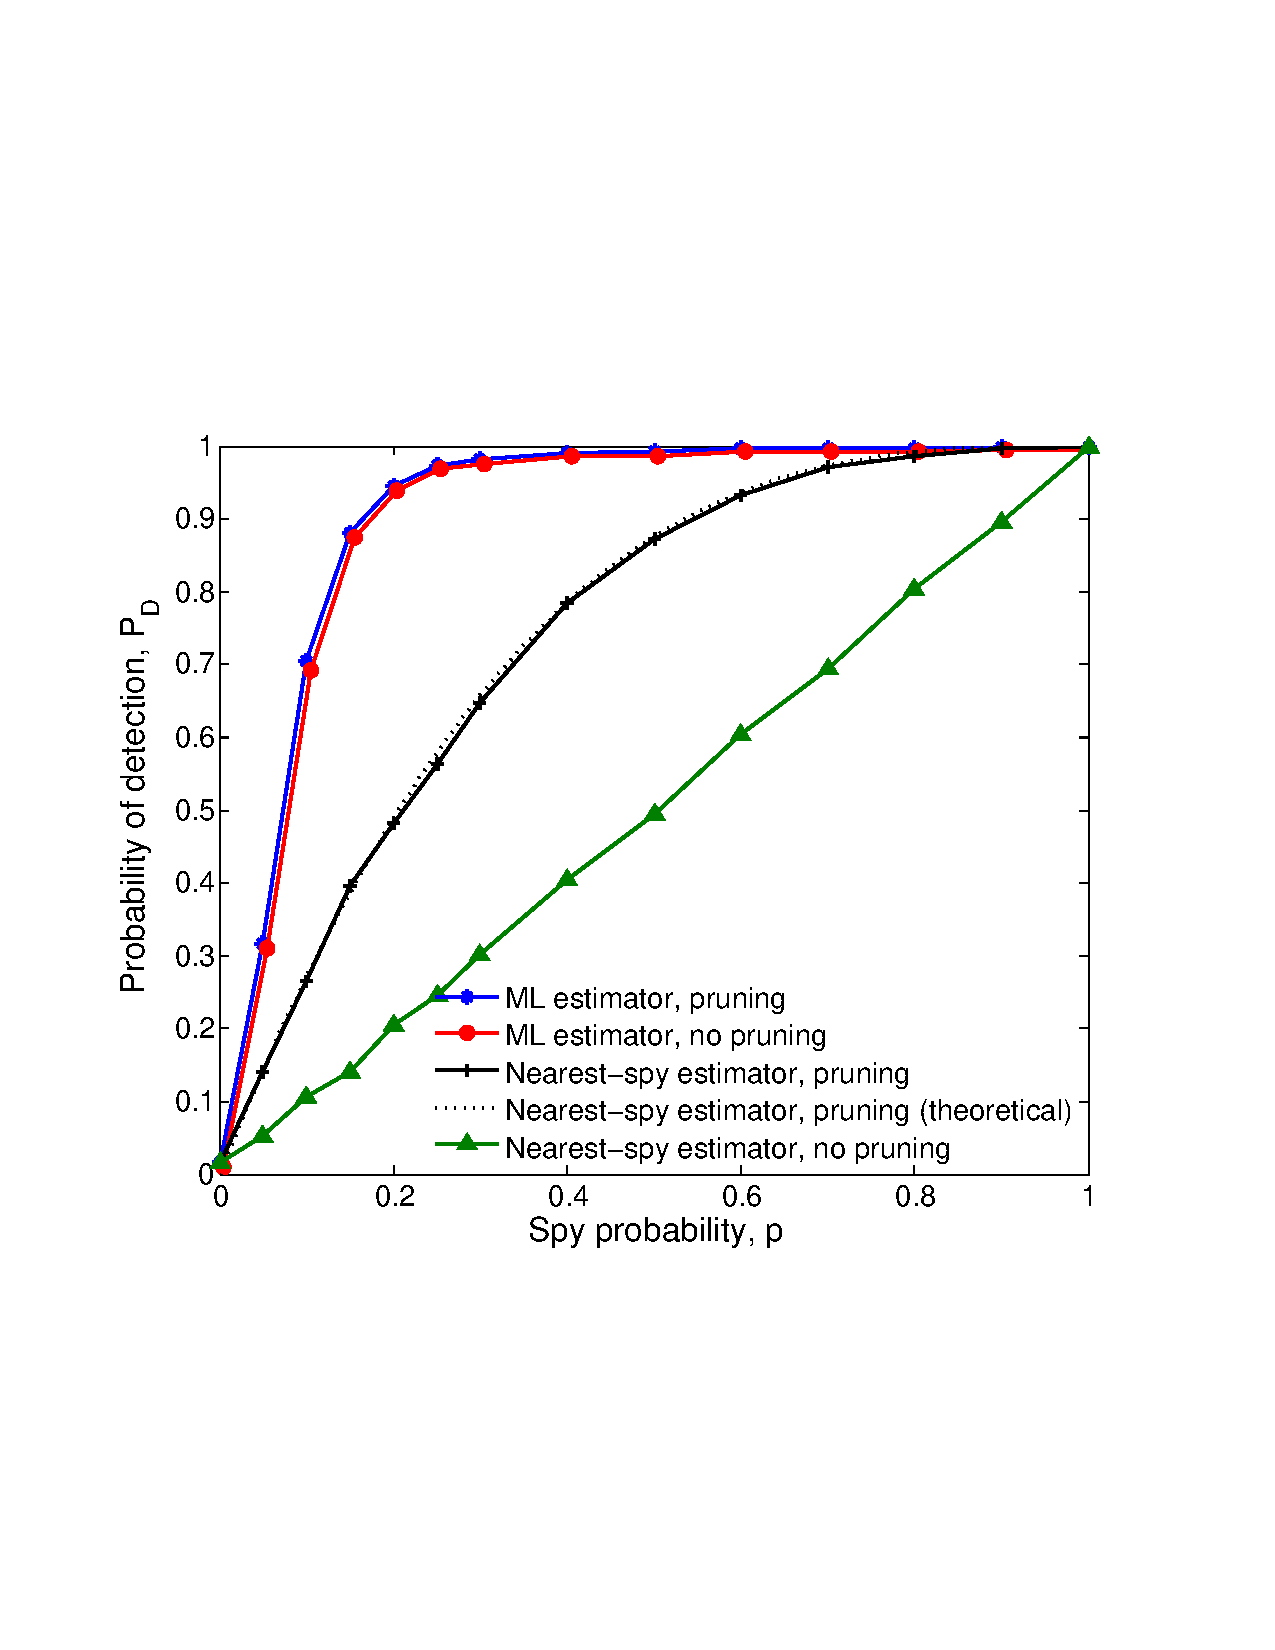
\includegraphics[height = 2.4in]{figures/pd_vs_spies}
\caption{Probability of detection, i.e. $P(\hat v = v^*)$, as a function of the spy probability $p$. This plot was generated over 3-regular trees. Delays $\theta_{ij}$ are modeled as Gaussians $\mathcal N(2,0.5)$, and spreading was run for 8 time units.}
\label{fig:pd_vs_spies}
%\vspace*{-0.4in}
\end{figure}

\begin{figure}
\centering
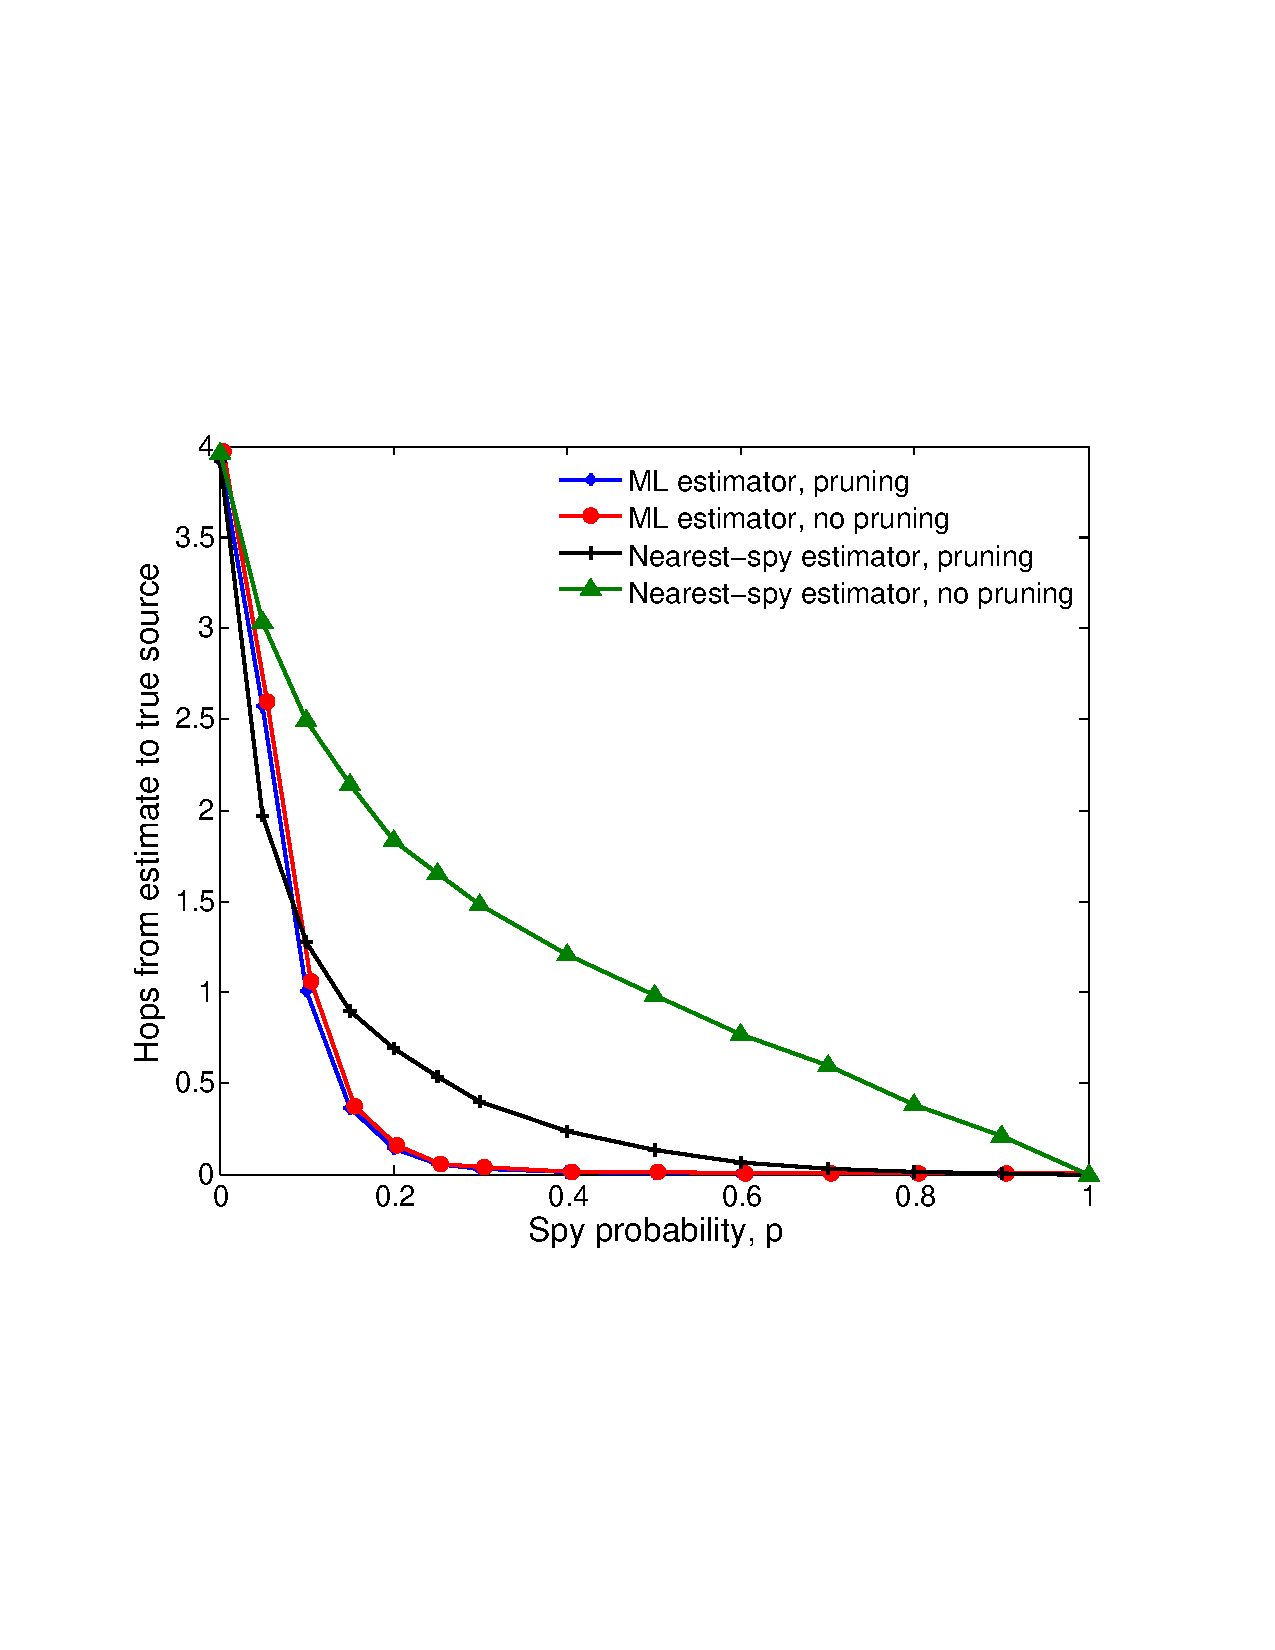
\includegraphics[height = 2.4in]{figures/hops_vs_spies}
\caption{Hop distance of the estimate $\hat v$ from the true source $v^*$ as a function of the spy probability $p$. This plot was generated over 3-regular trees. Delays $\theta_{ij}$ are modeled as Gaussians $\mathcal N(2,0.5)$, and spreading was run for 8 time units.}
\label{fig:pd_vs_spies}
%\vspace*{-0.4in}
\end{figure}


\bibliography{references}
\bibliographystyle{ieeetr}
\end{document}
